% !TeX spellcheck = en_GB 

\section{Physical properties of the problem}
\begin{frame}
\begin{block}{Thermal diffusivities}
\begin{align*}
\alpha_{cake}=&1.02\times 10^{-7} \SI{}{\meter/\second^2 } \text{ to } 1.698\times 10^{-7} \SI{}{\meter/\second^2}\\
\alpha_{Al} =&9.444\times 10^{-5} \SI{}{\meter/\second^2}\\
\end{align*}
\end{block}
\begin{block}{radius}
\begin{align*}
r_{cake} =& 15\SI{}{\centi\meter}
\end{align*}
\end{block}
\end{frame}

\begin{frame}
\frametitle{The Grid}
\begin{figure}[htp]
        \centering
        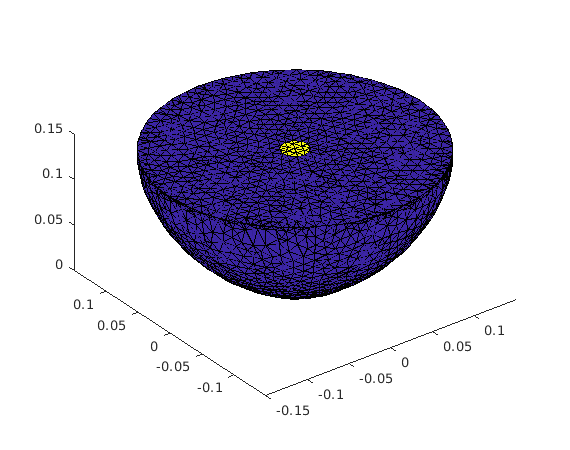
\includegraphics[width=0.8\textwidth]{figures/mesh.png}
\end{figure}
\end{frame}
